\chapter{Автономный генератор }
Дана система вида:
\[
    \begin{cases}
        \dot x = Ax \\
        g = Cx
    \end{cases} \quad x(0)
\]

Необходимо задать такие параметры \( A \), \( C \) и \(x(0)\),
чтобы выход системы при свободном движении совпадал с 
желаемым сигналом \( g_\text{ж}(t) = \sin(-5t) + e^{5t}cos(-5t)\)

Необходимо построить \( g_{\text{св}}(t) \) как:

\[
g_{\text{св}}(t) = C e^{At} x(0)
\]

Из желаемого сигнала находим нужные собственные значения:
\[
    \lambda_{1,2} = \pm 5i, \quad \lambda_{3,4} = 5 \pm 5i
\]

Составим Жорданову матрицу \( A \):
\[
    A = \begin{bmatrix}
        0 & 5 & 0 & 0 \\
        -5 & 0 & 0 & 0 \\
        0 & 0 & 5 & 5 \\
        0 & 0 & -5 & 5
    \end{bmatrix}
\]

Матричная экспонента от \( A \):
\[
    e^{At} = \begin{bmatrix}
        \cos(5t) & \sin(5t) & 0 & 0 \\
        -\sin(5t) & \cos(5t) & 0 & 0 \\
        0 & 0 & e^{5t}\cos(5t) & e^{5t}\sin(5t) \\
        0 & 0 & -e^{5t}\sin(5t) & e^{5t}\cos(5t)
    \end{bmatrix}
\]

Составим выражение для \( g_{\text{св}}(t) \):
\[
    g_{\text{св}}(t) = C e^{At} x(0)
\]
\[
    g_{\text{св}}(t) = 
    \begin{bmatrix}
        c_1 & c_2 & c_3 & c_4
    \end{bmatrix}
    \begin{bmatrix}
        \cos(5t) & \sin(5t) & 0 & 0 \\
        -\sin(5t) & \cos(5t) & 0 & 0 \\
        0 & 0 & e^{5t}\cos(5t) & e^{5t}\sin(5t) \\
        0 & 0 & -e^{5t}\sin(5t) & e^{5t}\cos(5t)
    \end{bmatrix} 
    \begin{bmatrix}
        x_1 \\
        x_2 \\
        x_3 \\
        x_4
    \end{bmatrix}
\]
\[
g_{\text{св}}(t) = \cos(-5t) \big(c_1 x_1 + c_2 x_2 + c_3 e^{5t} x_3 + c_4 e^{5t} x_4\big)
+
\]\[ 
+ \sin(-5t) \big(c_2 x_1 - c_1 x_2 - c_4 e^{5t} x_3 + c_3 e^{5t} x_4\big).
\]

Для того чтобы выход системы совпадал с желаемым сигналом, необходимо:
\[
    \begin{cases}
        c_1 x_1 + c_2 x_2 = 0 \\
        c_3  x_3 + c_4 x_4 = 1 \\
        c_2 x_1 - c_1 x_2 = 1 \\
        - c_4  x_3 + c_3 x_4 = 0
    \end{cases}
\]

Нам подойдут например следующие значения:
\[
    \begin{cases}
        c_1 = 0, \, c_2 = 1, \, c_3 = 0, \, c_4 = 1 \\
        x_1 = 1, \, x_2 = 0, \, x_3 = 0, \, x_4 = 1
    \end{cases}
\]

Получили значения для \( A \), \( C \) и \( x(0) \):
\[
    A = \begin{bmatrix}
        0 & 5 & 0 & 0 \\
        -5 & 0 & 0 & 0 \\
        0 & 0 & 5 & 5 \\
        0 & 0 & -5 & 5
    \end{bmatrix}, \quad
    C = \begin{bmatrix}
        0 & 1 & 0 & 1
    \end{bmatrix}, \quad
    x(0) = \begin{bmatrix}
        1 \\
        0 \\
        0 \\
        1
    \end{bmatrix}
\]
Создадим соответствующую систему в Simulink:
\begin{figure}[H]
    \centering
    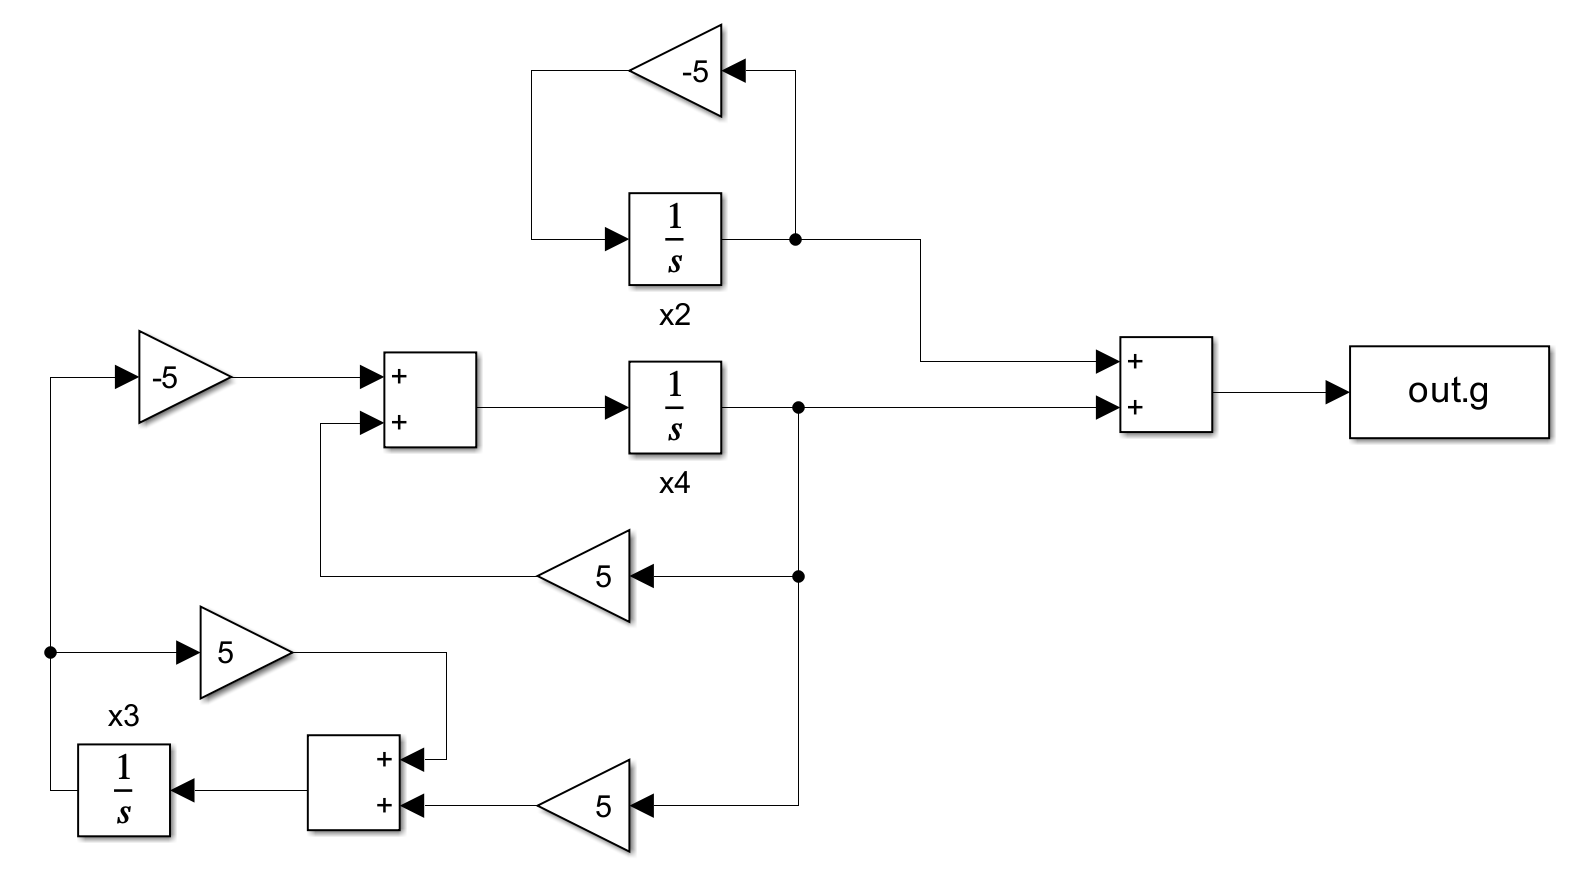
\includegraphics[width=1\textwidth]{../images/sim3.png}
    \caption{Система в Simulink}
\end{figure}
Сравним выход системы с желаемым сигналом:
\begin{figure}[H]
    \centering
    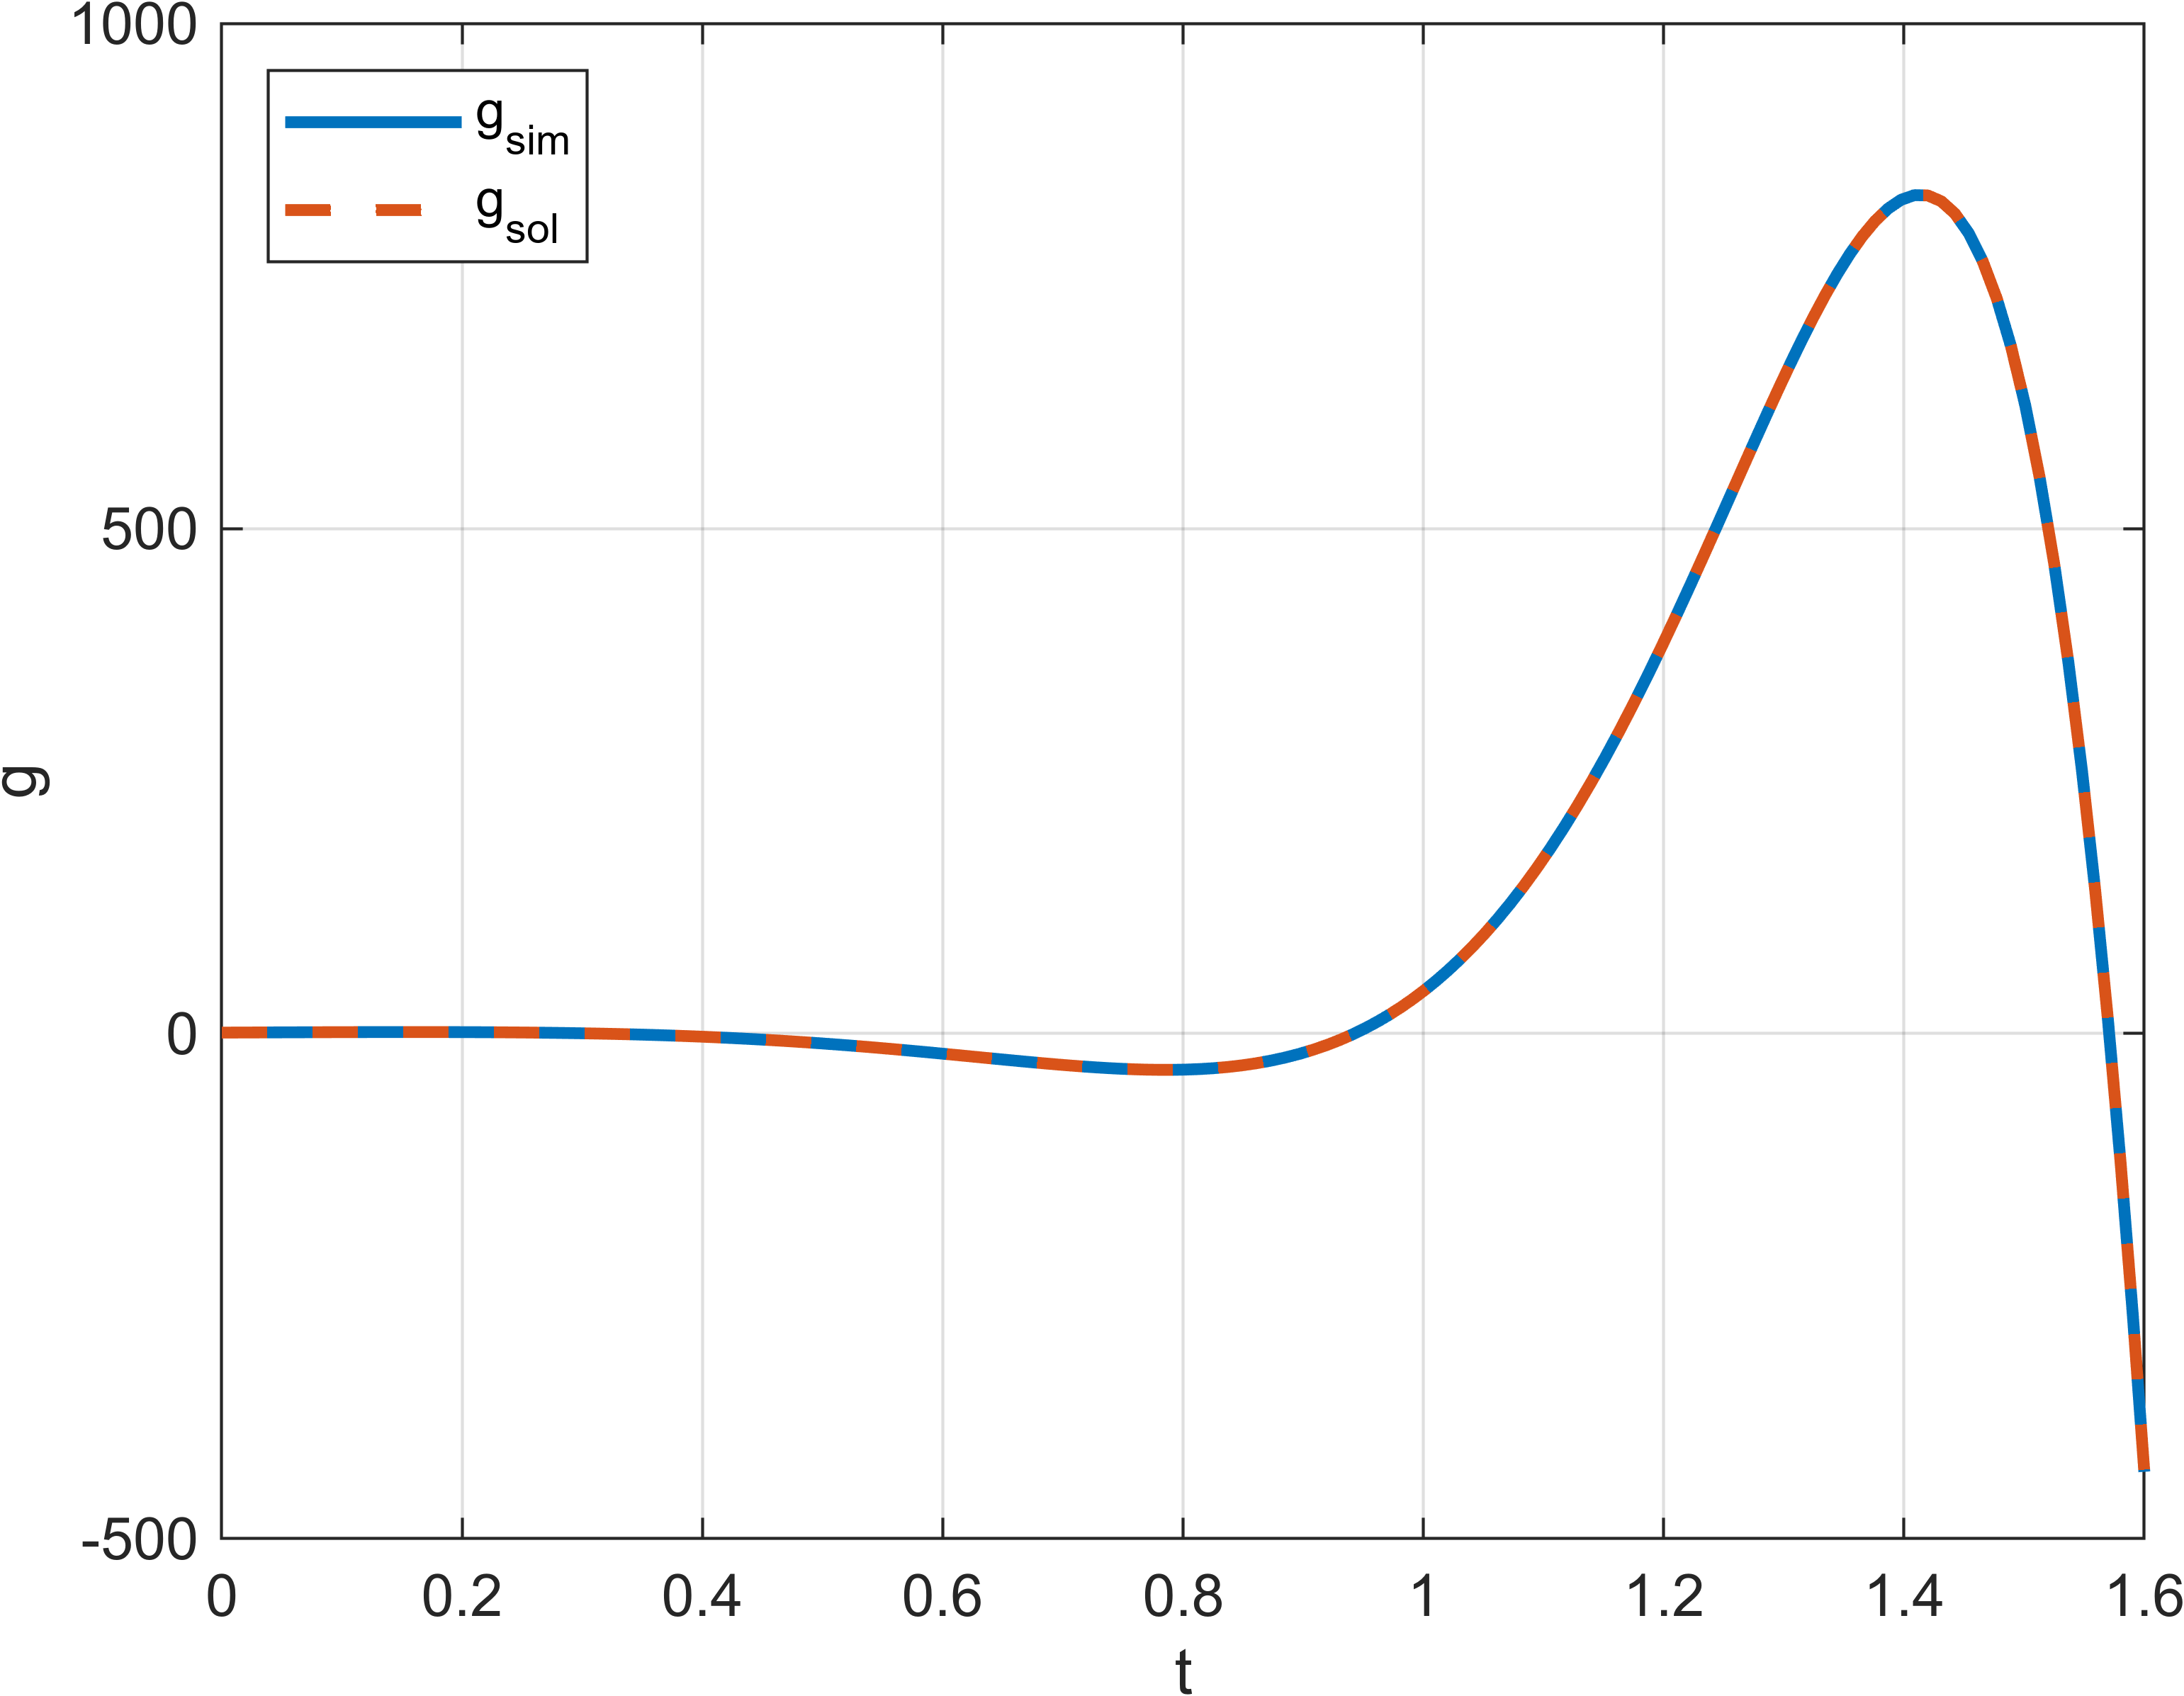
\includegraphics[width=1\textwidth]{../images/3_1.png}
    \caption{Сравнение выхода генератора с желаемым сигналом}
\end{figure}
\endinput